%% Chapter 7 %%%
\chapter{Регрессия к среднему и правила остановки}
\label{chp7}

Медицинские испытания недешевы. Чтобы обеспечить группу пациентов экспериментальными лекарствами и отслеживать проявления их симптомов на протяжении месяцев, может потребоваться значительное количество ресурсов, поэтому многие фармакологические компании разработали т.н. ``правила остановки'', которые позволяют исследователям остановить эксперимент заранее, если очевидно, что экспериментальное лекарство имело значительный эффект. Например, если эксперимент проведён только на половину, но у исследователей уже есть статистически значимые различия в симптомах от действия нового препарата - в таком случае, исследователи могут остановить эксперимент, не стремясь собрать больше данных для подкрепления своих выводов.

Однако, если исследование проведено плохо, это может привести к огромному количеству ложноположительных результатов. 

Например, представьте, что мы сравниваем две группы пациентов, одна их которых принимает лекарство, а другая - плацебо. Мы измеряем уровень какого-нибудь белка в их кровотоке, интерпретируя это как результат действия лекарства. Однако в этом случае, лекарство не вызывает никаких различий: пациенты обеих групп имеют одинаковый средний уровень белка, хотя, естественно, индивидуально уровни слегка различаются. 

Мы начинаем эксперимент с десятью пациентами в каждой группе, и постепенно собираем всё больше данных. В процессе эксперимента, мы проводим $t-$тест для сравнения двух групп и проверки наличия между ними статистически значимых различий в среднем уровне белка. Мы можем увидеть данные, схожие с результатами симуляции на рисунке ниже:


\newpage % делаем разрыв, чтобы картинка была первой на след странице

%%%%%%%%%%%%%% figure 9 %%%%%%%%%%%%%%%%%%5
\begin{figure}[h!]
    \centering
    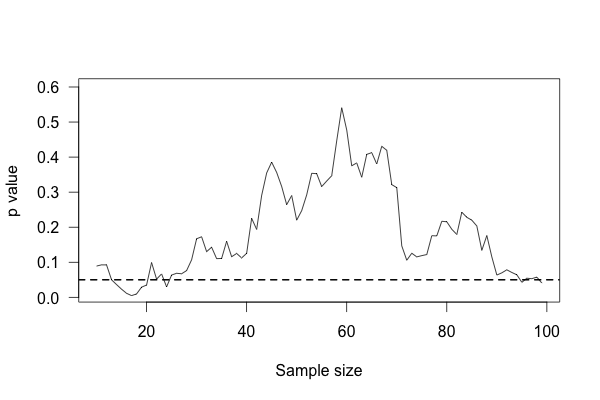
\includegraphics[width=0.8\textwidth]{sample-size}
    %\caption{}
    \label{fig9:sample-size}
\end{figure}
%%%%%%%%%%%%%%% end of figure %%%%%%%%%%%%%%%%%%%

Этот график показывает изменения \emph{p}-значения различий между группами в процессе сбора нами данных, а горизонтальная линия означает уровень значимости $p = 0,05$. На первый взгляд может показаться, что значимых различий нет. Тогда мы собираем больше данных и делаем противоположный вывод. Если бы мы решили остановиться, это было бы заблуждением: мы были бы убеждены в том, что между группами существует значимое различие, в то время как в реальности его нет. Если мы соберём еще больше данных, мы поймем, что были неправы - но в таком случае, есть шанс снова получить ложноположительный результат.  

Можно ожидать, что такое изменение \emph{p}-значения не должно происходить, поскольку реальных различий между группами нет. В конце концов, сбор большего количества данных не должно ухудшать наши выводы, разве нет? И действительно, если мы проведем эксперимент еще раз, мы можем обнаружить, что в начале у групп нет значимых различий, и они не появляются, пока мы собираем данные, или, что сначала у групп есть огромные различия, но в процессе эксперимента они быстро уменьшаются до нуля. Но если мы подождем достаточно долго и будем сравнивать различия после каждого измерения, в конечном итоге мы можем пересечь любую произвольную линию статистической значимости, даже если в реальности различий не будет. Обычно мы не в состоянии собирать данные на бесконечных выборках, поэтому в реальности такого не происходит, но неудачно  составленные и плохо применяемые правила остановки все равно значимо увеличивают количество ложноположительных результатов.\cite{simmons_false-positive_2011}  


Современные клинические испытания часто требуют регистрации используемых статистических протоколов заранее, и, как правило, выбирают только некоторые резальтаты измерения, которые потом тестируют, вместо того, чтобы тестировать после каждого измерения. Это вызывает лишь небольшое увеличение ложноположительных результатов, которое можно корректировать тщательно подобранными уровнями значимости и используя сложные статистические методы.\cite{todd_interim_2001} Но в сферах науки, где протоколы исследования не регистрируются и у исследователей есть возможность выбирать любые методы, которые они считают подходящими, всегда найдется место для таких ошибок.


\section{Преувеличение истины}
\label{chp7:truthinflation}

У медицинских экспериментов также существует тенденция иметь неадекватную статистическую мощность для определения умеренных различий между лекарствами. И они стремятся остановить исследование, как только обнаруживается какой-то результат, но у них не хватает мощности, чтобы обнаружить различия.

Предположим, что лекарство снижает проявление симптомов на 20\% по сравнению с плацебо, но эксперимент, в котором вы пытаетесь это проверить, не имеет адекватной статистической мощности, чтобы определить это различие. Мы знаем, что результаты небольших исследований могут варьировать: удачно собрать в одном эксперименте десять пациентов с более короткой продолжительностью простуды, чем в среднем, легко, но гораздо сложнее собрать десять тысяч таких людей.   

А теперь представьте, что вы проводите множество таких же экспериментов. Иногда вам попадаются не такие удачливые пациенты, и поэтому вы не замечаете никакого статистически значимого улучшения от действия вашего лекарства. Иногда пациенты имеют типично средние показатели, и можно рпонаблюдать снижение симптомов на 20\% благодаря лекарству, но вы игнорируете эти результаты, поскольку у вас недостаточно данных для того, чтобы считать такое улучшение статистически значимым. Иногда пациентам везёт, и их симптомы снижаются более, чем на 20\%, и тогда вы останавливаете эксперимент и говорите:``Смотрите! Лекарство работает!'' 

Вы правильно сделали вывод, что лекарство эффективно, но вы преувеличили размер эффекта. Вы ошибочно поверили в то, что лекарство более эффективно, чем оно есть на самом деле. 

Это часто встречается в фармакологических испытаниях, эпидемиологических исследованиях, исследованиях связей на генном уровне (``ген А является причиной условия В''), психологических исследованиях и в некоторых наиболее цитируемых статьях в медицинской литературе.\cite{ioannidis_why_2008,ioannidis_contradicted_2005} В сферах, где испытания могут проводиться быстро и большим количеством независимых исследователей (как, например, исследования генных связей), самые первые опубликованные результаты зачастую оказываются крайне противоречивыми, поскольку небольшие размеры экспериментов и потребность в статистической значимости приводят к тому, что лишь наиболее выдающиеся результаты в итоге публикуются.\cite{ioannidis_early_2005} 

В качестве бонуса, преувеличение истины можно объединять с правилами предварительной остановки. Если большинство лекарств в клинических испытаниях не настолько эффективны, чтобы оправдать предварительную остановку испытаний, в таком случае большинство экспериментов, остановленных предварительно, будут результатом участия удачливых пациентов, а не действия выдающихся лекарств, - и, останавливая эксперимент, мы фактически лишаем себя возможности собрать дополнительные данные, чтобы это опровергнуть. В обзорах научной литературы сравнивались исследования, остановленные предварительно, с другими, которые изучали те же вопросы, но не были предварительно остановлены, и в большинстве случаев, в предварительно остановленных исследованиях эффект действия тестируемых лекарств был в среднем преувеличен на 29\%.\cite{bassler_stopping_2010} 

Естественно, нам неизвестна ``Истина'' о каждом исследуемом лекарстве, поэтому сложно судить, было ли конкретное исследование предварительно остановлено из-за хорошего лекарства или по желанию исследователей. Во многих исследованиях даже не публикуется изначально планируемый размер выборки или правила остановки, используемые для обоснования прекращения исследования.\cite{montori_randomized_2005} Предварительная остановка исследования не свидетельствует автоматически о том, что его результаты ошибочны, но это определенно наводит на мысль.  



\section{Маленькие крайности}
\label{chp7:littleextremes}

Предположим, что вы ответственны за проведение реформы государственных школ. В рамках изучениях лучших методов обучения, вы обратили внимание на влияние размера школы на результаты тестирования учеников. Лучше ли результаты у маленьких школ, чем у больших? Стоит ли построить большое количество небольших школ или лучше несколько больших?   

Чтобы найти ответы на эти вопросы, вы составляете список лучших школ. В среднем, в школе около 1000 учеников, но практически во всех школах, входящих в десятку лучших по списку, учеников меньше. Похоже, что маленькие школы справляются с обучением лучше, возможно из-за того, что в них формируются условия, при которых учителям удаётся получше узнать учеников и помогать им в индивидуальном порядке.

Затем вы смотрите на худшие из списка школы, ожидая увидеть там большие городские школы с тысячами учеников и перегруженными работой учителями, однако, к вашему удивлению, и там все школы маленькие. 

Что же происходит? Давайте посмотрим на график зависимости результатов тестирования от размера школ:


%\newpage % делаем разрыв, чтобы картинка была первой на след странице

%%%%%%%%%%%%%% figure 10 %%%%%%%%%%%%%%%%%%5
\begin{figure}[h!]
    \centering
    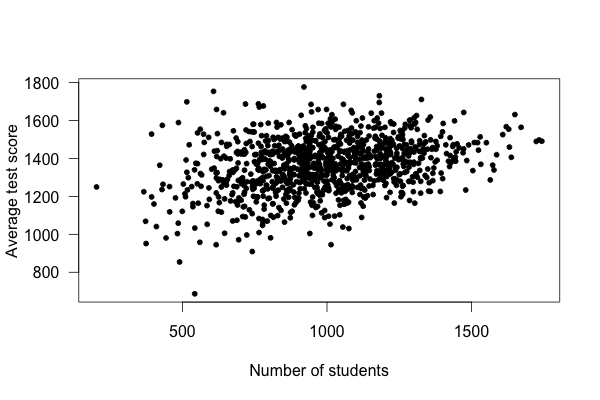
\includegraphics[width=0.8\textwidth]{school-size}
    %\caption{}
    \label{fig9:school-size}
\end{figure}
%%%%%%%%%%%%%%% end of figure %%%%%%%%%%%%%%%%%%%
%%%%%%%%%%%%%%%%%%%%%%%%%%%55
%http://www.statisticsdonewrong.com/_images/school-size.png
%%%%%%%%%%%%%%%%%%%%%%%%%%%%%%%%

У маленьких школ средние значения результатов тестирования значительно варьируются, в основном из-за того, что у них меньше учеников. Меньшее количество учеников означает меньшее наличие данных для того, чтобы установить ``истинные'' результаты работы учителей, и поэтому средние значения результатов сильно разнятся. Чем крупнее школа, тем меньше варьируют результаты, а среднее значение, в действительности, даже увеличивается.  

В этом примере использовались данные симуляции, но он основан на настоящих (и неожиданных) результатах наблюдения за государственными школами Пенсильвании.\cite{wainer_most_2007}

Другой пример: В Соединенных Штатах, наименьший уровень заболевания раком почки, как правило, имеют сельские округа Среднего Запада, а также южные и западные штаты. Почему так? Можно найти несколько объяснений, например: деревенские жители больше заняты физическим трудом, дышат менее загрязненным воздухом и, возможно, ведут менее напряженный образ жизни. Вероятно, эти факторы снижают показатели встречаемости рака. 

С другой стороны, округа с самыми высоким уровнем заболевания раком почки выступают те же сельские округа Среднего Запада, южные и западные штаты.

Проблема, естественно, заключает в том, что в сельской местности живёт меньше людей. Единственный пациент с диагнозом рака почки в округе, где живет всего 10 человек, даст этому округу самый высокий уровень заболевания раком почки по всей стране. Следовательно, маленькие округа имеют значительно более варьируемые показатели заболевания раком почки, просто потому, что у них так мало жителей.\cite{gelman_all_1999}

